\documentclass[10pt,letterpaper,twocolumn]{article}
\usepackage[T1]{fontenc}
\usepackage[margin=0.8in,columnsep=0.25in]{geometry}
\usepackage{libertine,amsmath,amssymb,booktabs,tabularx,array,tikz,fvextra}
\usepackage{iftex}
\ifPDFTeX\else
\usepackage{unicode-math}
\setmathfont{LibertinusMath-Regular.otf}
\fi
\usepackage[numbers]{natbib}
\usepackage[hidelinks]{hyperref}
\usepackage{xurl}
\newcommand{\Description}[1]{} % Accessibility descriptions retained in source.
\setlength{\emergencystretch}{1em}
\title{How Much of the Organization Should Agents Know? The Marginal Value of Global Topology Awareness in Hierarchical Multi-Agent Systems}
% Author details supplied by the author on 14 October 2026.
\author{Haoyan Xu\\[0.4em]
\small China University of Geosciences (Beijing)\\
\small \href{mailto:xuhaoyan800@gmail.com}{\texttt{xuhaoyan800@gmail.com}}}

\date{Preprint --- 14 October 2026}
\hypersetup{pdftitle={How Much of the Organization Should Agents Know? The Marginal Value of Global Topology Awareness in Hierarchical Multi-Agent Systems},pdfauthor={Haoyan Xu}}
\begin{document}
\twocolumn[\begin{@twocolumnfalse}
\maketitle
\begin{abstract}

Hierarchical multi-agent sys\-tems can maintain or\-ga\-ni\-za\-tions that their individual agents never see in full. Native role instructions and local in\-ter\-faces reveal partial or\-ga\-ni\-za\-tion\-al views, yet these views can be sufficient for coordinated ex\-e\-cu\-tion. How a broad\-er or\-ga\-ni\-za\-tion\-al view changes par\-tic\-i\-pa\-tion in an already functioning or\-ga\-ni\-za\-tion remains unclear. We investigate or\-ga\-ni\-za\-tion\-al vis\-i\-bil\-i\-ty in paired experiments with ROMA and TalkHier, presenting mod\-els with a stat\-ic account of their ex\-ist\-ing roles, relationships, and in\-for\-ma\-tion flows while preserving na\-tive ex\-e\-cu\-tion mech\-a\-nisms. The behavioral responses differ markedly. ROMA reduces re\-cur\-sive ex\-pan\-sion by 16--19\% across two ques\-tion-an\-swer\-ing settings, whereas TalkHier increases expert par\-tic\-i\-pa\-tion and in\-ter\-nal analysis, using 65\% more normal-return tokens. Task out\-comes do not mirror these changes: SEAL-0 changes little, FRAMES shows a favorable but un\-cer\-tain im\-prove\-ment, and MMLU-Pro Phys\-ics improves slightly. Recorded repeat success and external col\-lab\-o\-ra\-tion ratings also show little ac\-com\-pa\-ny\-ing im\-prove\-ment. These findings show that or\-ga\-ni\-za\-tion\-al vis\-i\-bil\-i\-ty can reshape how an ex\-ist\-ing or\-ga\-ni\-za\-tion operates without consistently improving its task out\-comes or com\-pu\-ta\-tion\-al efficiency. Organizational in\-for\-ma\-tion completeness and practical utility are distinct properties.

\end{abstract}
\noindent\textbf{Keywords:} Hierarchical multi-agent systems, organizational visibility, LLM agents, empirical evaluation
\vspace{1.2em}
\end{@twocolumnfalse}]
\section{Introduction}
A multi-agent sys\-tem can enforce an or\-ga\-ni\-za\-tion without making that or\-ga\-ni\-za\-tion fully visible to its agents. In hierarchical LLM sys\-tems, the program assigns roles, constrains communication routes, delegates tasks, and carries results back through the relevant relationships. An individual mod\-el encounters its own functional or role instructions, selected upstream or downstream in\-ter\-faces, and con\-text associated with its current work. The or\-ga\-ni\-za\-tion maintained by the sys\-tem and the or\-ga\-ni\-za\-tion\-al view supplied to a member are therefore distinct. Recursive del\-e\-ga\-tion in ROMA and nested supervision in TalkHier exemplify this separation between implementing an or\-ga\-ni\-za\-tion and making it visible \cite{roma,talkhier}.

Members receive a \textbf{partial, lossy or\-ga\-ni\-za\-tion\-al view}. Remote responsibilities, relationships across branches, and complete return paths can remain at the sys\-tem level without appearing together in a mod\-el input. This view can be functionally sufficient: local instructions and programmed coordination already allow the or\-ga\-ni\-za\-tion to operate. \textbf{Functional sufficiency does not establish informational adequacy.} Here, “lossy” denotes nondisclosure of some or\-ga\-ni\-za\-tion\-al in\-for\-ma\-tion; its value for par\-tic\-i\-pa\-tion remains an empirical ques\-tion.

As responsibilities span more roles, levels, and branches, the distinction between local and global or\-ga\-ni\-za\-tion\-al vis\-i\-bil\-i\-ty becomes a concrete design choice. Existing research treats topo\-lo\-gy, role as\-sign\-ment, and rules as components of or\-ga\-ni\-za\-tion\-al prompts \cite{guoorganized}, while hierarchical frame\-works distribute planning, ex\-e\-cu\-tion, and review across dif\-fer\-ent positions \cite{massurvey,orgagent,institutions}. A broad\-er or\-ga\-ni\-za\-tion\-al view can place a member's local responsibilities within the overall division of work and reveal where contributions travel and return. This in\-for\-ma\-tion could help members anticipate col\-lab\-o\-ra\-tion, change del\-e\-ga\-tion strategies, or commit more effort to particular roles. What remains unclear is how these possibilities affect an or\-ga\-ni\-za\-tion that already coordinates work through its na\-tive in\-ter\-faces. \textbf{When members gain access to a broad\-er or\-ga\-ni\-za\-tion\-al view, how does their par\-tic\-i\-pa\-tion in that or\-ga\-ni\-za\-tion change?}

We examine this ques\-tion by separating or\-ga\-ni\-za\-tion\-al implementation from or\-ga\-ni\-za\-tion\-al vis\-i\-bil\-i\-ty. We compare BASE, with each system's native organizational context, and ORG-DESC, with a global static account of the existing roles, relationships, and information flows. We implement this vis\-i\-bil\-i\-ty con\-trast through or\-ga\-ni\-za\-tion\-al de\-scrip\-tions in mod\-el con\-text, keeping the na\-tive roles, tools, routing in\-ter\-faces, and ex\-e\-cu\-tion rules fixed. The experiments cover ROMA on SEAL-0 and FRAMES and TalkHier on MMLU-Pro Phys\-ics. Their na\-tive views differ, so the paired comparisons estimate changes within each ar\-chi\-tec\-ture's informational and ex\-e\-cu\-tion setting.

Organizational vis\-i\-bil\-i\-ty reshapes ex\-e\-cu\-tion in dif\-fer\-ent ways. ROMA reduces re\-cur\-sive ex\-pan\-sion by 16--19\% across its two ques\-tion-an\-swer\-ing settings. TalkHier keeps its role hierarchy while broadening expert participation and increasing work inside role invocations, using 65\% more normal-return tokens. These behavioral changes have no simple correspondence with task value: SEAL-0's mean utility barely changes, FRAMES has a favorable but un\-cer\-tain estimate of +8.51 percentage points, and TalkHier improves slightly. Recorded repeat success and external col\-lab\-o\-ra\-tion ratings also change little. The contrasting responses show that a broad\-er or\-ga\-ni\-za\-tion\-al view can change how agents collaborate while its task benefits and com\-pu\-ta\-tion\-al con\-se\-quences depend on the setting.

This paper makes three contributions. First, it separates the or\-ga\-ni\-za\-tion implemented by a sys\-tem from the or\-ga\-ni\-za\-tion\-al view available to its members, and operationalizes vis\-i\-bil\-i\-ty under preserved ex\-e\-cu\-tion mech\-a\-nisms. Second, it characterizes contrasting ex\-e\-cu\-tion responses through complete re\-cur\-sive task trees and role-level traces, distinguishing del\-e\-ga\-tion, role par\-tic\-i\-pa\-tion, and work within a visit. Third, it eval\-u\-ates these responses through task out\-comes, re\-cord\-ed repeat success, com\-pu\-ta\-tion\-al work, and external col\-lab\-o\-ra\-tion ratings. Together, these results establish or\-ga\-ni\-za\-tion\-al vis\-i\-bil\-i\-ty as a design variable whose behavioral effects and practical value require separate evaluation.

\section{Related Work}
\textbf{Organizational mech\-a\-nisms.} Multi-agent ar\-chi\-tec\-tures specify who performs which work, which members may communicate, and how intermediate results are coordinated. Surveys distinguish centralized, decentralized, hierarchical, and shared-in\-for\-ma\-tion configurations \cite{massurvey}. ROMA builds task or\-ga\-ni\-za\-tions recursively through a reused processing template, while TalkHier organizes generation, evaluation, and revision through nested teams \cite{roma,talkhier}. OrgAgent and institution-oriented approaches extend the design space to differentiated governance, ex\-e\-cu\-tion, review, and decision authority \cite{orgagent,institutions}. These studies treat or\-ga\-ni\-za\-tion\-al structure as a substantive design variable. We examine or\-ga\-ni\-za\-tion\-al vis\-i\-bil\-i\-ty while preserving the na\-tive or\-ga\-ni\-za\-tion\-al mech\-a\-nisms.

\textbf{Organizational in\-for\-ma\-tion.} Role de\-scrip\-tions, named team rosters, routing schemas, and selected histories already convey or\-ga\-ni\-za\-tion\-al in\-for\-ma\-tion to mod\-els. Guo et al.'s topo\-lo\-gy--\allowbreak{}role as\-sign\-ment--\allowbreak{}rules classification makes this informational content explicit, and their or\-ga\-ni\-za\-tion\-al prompts shape embodied cooperation \cite{guoorganized}. Organizational de\-scrip\-tions can thus help establish its behavior. In a programmatically orchestrated sys\-tem, the mech\-a\-nism can remain fixed while the member-visible view changes. Experiments that jointly vary roles, routing, and or\-ga\-ni\-za\-tion\-al prompts leave these two dimensions coupled. Our comparison expands vis\-i\-bil\-i\-ty from each sys\-tem's na\-tive con\-text to a global stat\-ic or\-ga\-ni\-za\-tion\-al account while retaining the same ex\-e\-cu\-tion in\-ter\-faces.

\textbf{Evaluating realized col\-lab\-o\-ra\-tion.} Answer scores summarize task out\-comes but leave open how an or\-ga\-ni\-za\-tion produced them. Task trees cap\-ture re\-cur\-sive del\-e\-ga\-tion; role-level traces cap\-ture visits and work within a visit. Tree edit distance compares complete tree structures beyond scalar depth or node counts \cite{apted}. MultiAgentBench supplies external planning and communication rubrics through MARBLE \cite{mab}, complementing direct ex\-e\-cu\-tion mea\-sures with mod\-el-based assessments of re\-cord\-ed col\-lab\-o\-ra\-tion. These mea\-sures serve dif\-fer\-ent purposes: ex\-e\-cu\-tion re\-cords establish behavioral responses, out\-comes and resources evaluate their value, and external ratings provide a secondary perspective. Struc\-tur\-al-out\-come analyses remain supporting evidence rather than a separate mech\-a\-nism-dis\-cov\-ery objective.

\section{Organizational Views and Intervention}
\subsection{Implemented or\-ga\-ni\-za\-tion and visible view}
Let an implemented or\-ga\-ni\-za\-tion comprise role or functional contracts, allowed del\-e\-ga\-tion and routing, and result-handling rules. For a mod\-el call, its or\-ga\-ni\-za\-tion\-al view is the in\-for\-ma\-tion about that or\-ga\-ni\-za\-tion actually included in the input. A route in a graph or a role label in callback metadata does not by itself establish mod\-el vis\-i\-bil\-i\-ty. Native views can disclose some in\-for\-ma\-tion explicitly and other in\-for\-ma\-tion conditionally through the current task, available results, or selected history.

Local views need not be restricted to a single neighboring member, and they may contain the overall task objective. They are partial because they do not uniformly present the full or\-ga\-ni\-za\-tion\-al account. We therefore audit the actual input construction rather than assign a common vis\-i\-bil\-i\-ty percentage to the sys\-tems. The or\-ga\-ni\-za\-tion may also be generated during ex\-e\-cu\-tion: ROMA's stat\-ic processing template can be described globally even though the concrete future task tree does not yet exist.

\subsection{Two or\-ga\-ni\-za\-tions and their na\-tive in\-for\-ma\-tion boundaries}
Figure~\ref{fig:views} annotates nodes in both or\-ga\-ni\-za\-tion\-al schematics with their na\-tive in\-for\-ma\-tion. ROMA's nodes are tasks at dif\-fer\-ent re\-cur\-sive depths. Atomizer, Planner, Executor, and Aggregator are reused functional modules, not four management levels. Below the depth cap, atomization can choose direct ex\-e\-cu\-tion or planning. Planning creates subtasks and dependencies; child tasks reuse the processing mech\-a\-nism; aggregation integrates their results. At the cap, the program forces direct ex\-e\-cu\-tion. Native con\-texts include the current goal, overall objective, depth and limit, functional instructions, and module-specific results when available. The mod\-el therefore receives con\-text for its current re\-cur\-sive task without necessarily seeing the complete task tree.

TalkHier Phys\-ics instead starts from a configured six-role hi\-er\-ar\-chy. Default Supervisor selects among Answer Generator, Revisor, and Evaluator Supervisor; the latter selects Phys\-ics or Mathematics. A selected member returns through its supervisor. Default Supervisor receives its direct roster, job list, and dispatch choices; Evaluator Supervisor receives its experts and evaluation responsibilities. A leaf expert receives its own instructions, task background, and selected feedback history rather than a uniform de\-scrip\-tion of all six roles. These are role-centered local views of a fixed or\-ga\-ni\-za\-tion. The figure describes the Phys\-ics configuration used here; other TalkHier benchmark domains have dif\-fer\-ent expert sets and must not be assigned the same six-role map.

\begin{figure*}[t]
\centering

\resizebox{\linewidth}{!}{%
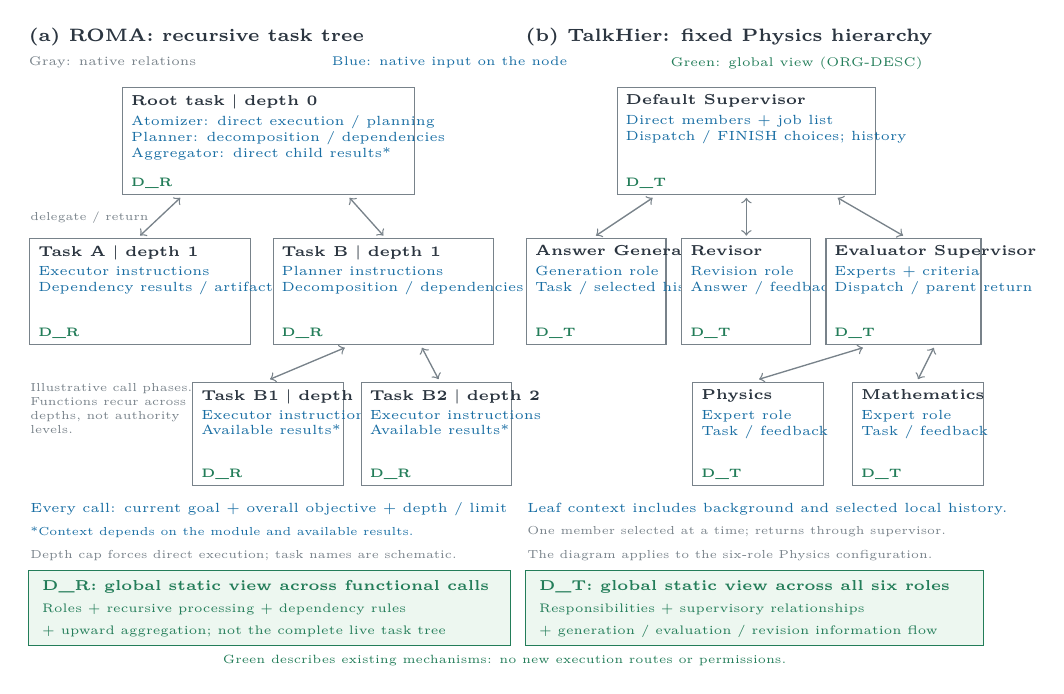
\begin{tikzpicture}[x=1cm,y=.80cm,every node/.style={inner sep=0pt}]
\definecolor{archgray}{HTML}{78828A}
\definecolor{archdark}{HTML}{2B3540}
\definecolor{archblue}{HTML}{176DA3}
\definecolor{archgreen}{HTML}{237D59}
\definecolor{archlightgray}{HTML}{F5F6F7}
\definecolor{archlightblue}{HTML}{EDF5FB}
\definecolor{archlightgreen}{HTML}{EDF7F0}
\node[anchor=north west,align=left,text=archdark,font=\fontsize{6.48}{7.78}\selectfont\bfseries] at (0.250,10.160) {(a) ROMA: re\-cur\-sive task tree};
\node[anchor=north west,align=left,text=archdark,font=\fontsize{6.48}{7.78}\selectfont\bfseries] at (6.560,10.160) {(b) TalkHier: fixed Phys\-ics hi\-er\-ar\-chy};
\node[anchor=north west,align=left,text=archgray,font=\fontsize{4.56}{5.47}\selectfont] at (0.250,9.700) {Gray: na\-tive relations};
\node[anchor=north west,align=left,text=archblue,font=\fontsize{4.56}{5.47}\selectfont] at (4.100,9.700) {Blue: na\-tive input on the node};
\node[anchor=north west,align=left,text=archgreen,font=\fontsize{4.56}{5.47}\selectfont] at (8.400,9.700) {Green: global view (ORG-\allowbreak{}DESC)};
\draw[draw=archgray,fill=white,line width=0.44pt] (1.450,7.500) rectangle (5.150,9.200);
\node[anchor=north west,align=left,text=archdark,font=\fontsize{5.20}{6.24}\selectfont\bfseries] at (1.550,9.100) {Root task | depth 0};
\node[anchor=north west,align=left,text=archblue,font=\fontsize{4.80}{5.76}\selectfont] at (1.550,8.770) {Atomizer: direct ex\-e\-cu\-tion / planning\\Planner: decomposition / dependencies\\Aggregator: direct child results*};
\node[anchor=north west,align=left,text=archgreen,font=\fontsize{4.44}{5.33}\selectfont\bfseries] at (1.550,7.770) {D\_R};
\draw[draw=archgray,fill=white,line width=0.44pt] (0.270,5.120) rectangle (3.070,6.800);
\node[anchor=north west,align=left,text=archdark,font=\fontsize{5.20}{6.24}\selectfont\bfseries] at (0.370,6.700) {Task A | depth 1};
\node[anchor=north west,align=left,text=archblue,font=\fontsize{4.80}{5.76}\selectfont] at (0.370,6.370) {Executor instructions\\Dependency results / artifacts*};
\node[anchor=north west,align=left,text=archgreen,font=\fontsize{4.44}{5.33}\selectfont\bfseries] at (0.370,5.390) {D\_R};
\draw[draw=archgray,fill=white,line width=0.44pt] (3.360,5.120) rectangle (6.160,6.800);
\node[anchor=north west,align=left,text=archdark,font=\fontsize{5.20}{6.24}\selectfont\bfseries] at (3.460,6.700) {Task B | depth 1};
\node[anchor=north west,align=left,text=archblue,font=\fontsize{4.80}{5.76}\selectfont] at (3.460,6.370) {Planner instructions\\Decomposition / dependencies};
\node[anchor=north west,align=left,text=archgreen,font=\fontsize{4.44}{5.33}\selectfont\bfseries] at (3.460,5.390) {D\_R};
\draw[draw=archgray,fill=white,line width=0.44pt] (2.340,2.880) rectangle (4.250,4.520);
\node[anchor=north west,align=left,text=archdark,font=\fontsize{5.20}{6.24}\selectfont\bfseries] at (2.440,4.420) {Task B1 | depth 2};
\node[anchor=north west,align=left,text=archblue,font=\fontsize{4.80}{5.76}\selectfont] at (2.440,4.090) {Executor instructions\\Available results*};
\node[anchor=north west,align=left,text=archgreen,font=\fontsize{4.44}{5.33}\selectfont\bfseries] at (2.440,3.150) {D\_R};
\draw[draw=archgray,fill=white,line width=0.44pt] (4.480,2.880) rectangle (6.390,4.520);
\node[anchor=north west,align=left,text=archdark,font=\fontsize{5.20}{6.24}\selectfont\bfseries] at (4.580,4.420) {Task B2 | depth 2};
\node[anchor=north west,align=left,text=archblue,font=\fontsize{4.80}{5.76}\selectfont] at (4.580,4.090) {Executor instructions\\Available results*};
\node[anchor=north west,align=left,text=archgreen,font=\fontsize{4.44}{5.33}\selectfont\bfseries] at (4.580,3.150) {D\_R};
\draw[<->,draw=archgray,line width=.48pt] (2.180,7.450)--(1.670,6.850);
\draw[<->,draw=archgray,line width=.48pt] (4.330,7.450)--(4.760,6.850);
\draw[<->,draw=archgray,line width=.48pt] (4.270,5.070)--(3.320,4.570);
\draw[<->,draw=archgray,line width=.48pt] (5.250,5.070)--(5.460,4.570);
\node[anchor=north west,align=left,text=archgray,font=\fontsize{4.16}{4.99}\selectfont] at (0.270,7.240) {delegate / return};
\node[anchor=north west,align=left,text=archgray,font=\fontsize{4.20}{5.04}\selectfont] at (0.270,4.510) {Illustrative call phases.\\Functions recur across\\depths, not authority\\levels.};
\node[anchor=north west,align=left,text=archblue,font=\fontsize{4.80}{5.76}\selectfont] at (0.270,2.620) {Every call: current goal + overall objective + depth / limit};
\node[anchor=north west,align=left,text=archblue,font=\fontsize{4.20}{5.04}\selectfont] at (0.270,2.240) {*Context depends on the module and available results.};
\node[anchor=north west,align=left,text=archgray,font=\fontsize{4.20}{5.04}\selectfont] at (0.270,1.870) {Depth cap forces direct ex\-e\-cu\-tion; task names are schematic.};
\draw[draw=archgray,fill=white,line width=0.44pt] (7.730,7.500) rectangle (11.010,9.200);
\node[anchor=north west,align=left,text=archdark,font=\fontsize{5.20}{6.24}\selectfont\bfseries] at (7.830,9.100) {Default Supervisor};
\node[anchor=north west,align=left,text=archblue,font=\fontsize{4.80}{5.76}\selectfont] at (7.830,8.770) {Direct members + job list\\Dispatch / FINISH choices; history};
\node[anchor=north west,align=left,text=archgreen,font=\fontsize{4.44}{5.33}\selectfont\bfseries] at (7.830,7.770) {D\_T};
\draw[draw=archgray,fill=white,line width=0.44pt] (6.580,5.120) rectangle (8.350,6.800);
\node[anchor=north west,align=left,text=archdark,font=\fontsize{5.20}{6.24}\selectfont\bfseries] at (6.680,6.700) {Answer Generator};
\node[anchor=north west,align=left,text=archblue,font=\fontsize{4.80}{5.76}\selectfont] at (6.680,6.370) {Generation role\\Task / selected history};
\node[anchor=north west,align=left,text=archgreen,font=\fontsize{4.44}{5.33}\selectfont\bfseries] at (6.680,5.390) {D\_T};
\draw[draw=archgray,fill=white,line width=0.44pt] (8.550,5.120) rectangle (10.180,6.800);
\node[anchor=north west,align=left,text=archdark,font=\fontsize{5.20}{6.24}\selectfont\bfseries] at (8.650,6.700) {Revisor};
\node[anchor=north west,align=left,text=archblue,font=\fontsize{4.80}{5.76}\selectfont] at (8.650,6.370) {Revision role\\Answer / feedback};
\node[anchor=north west,align=left,text=archgreen,font=\fontsize{4.44}{5.33}\selectfont\bfseries] at (8.650,5.390) {D\_T};
\draw[draw=archgray,fill=white,line width=0.44pt] (10.380,5.120) rectangle (12.350,6.800);
\node[anchor=north west,align=left,text=archdark,font=\fontsize{5.20}{6.24}\selectfont\bfseries] at (10.480,6.700) {Evaluator Supervisor};
\node[anchor=north west,align=left,text=archblue,font=\fontsize{4.80}{5.76}\selectfont] at (10.480,6.370) {Experts + criteria\\Dispatch / parent return};
\node[anchor=north west,align=left,text=archgreen,font=\fontsize{4.44}{5.33}\selectfont\bfseries] at (10.480,5.390) {D\_T};
\draw[draw=archgray,fill=white,line width=0.44pt] (8.690,2.880) rectangle (10.350,4.520);
\node[anchor=north west,align=left,text=archdark,font=\fontsize{5.20}{6.24}\selectfont\bfseries] at (8.790,4.420) {Phys\-ics};
\node[anchor=north west,align=left,text=archblue,font=\fontsize{4.80}{5.76}\selectfont] at (8.790,4.090) {Expert role\\Task / feedback};
\node[anchor=north west,align=left,text=archgreen,font=\fontsize{4.44}{5.33}\selectfont\bfseries] at (8.790,3.150) {D\_T};
\draw[draw=archgray,fill=white,line width=0.44pt] (10.720,2.880) rectangle (12.380,4.520);
\node[anchor=north west,align=left,text=archdark,font=\fontsize{5.20}{6.24}\selectfont\bfseries] at (10.820,4.420) {Mathematics};
\node[anchor=north west,align=left,text=archblue,font=\fontsize{4.80}{5.76}\selectfont] at (10.820,4.090) {Expert role\\Task / feedback};
\node[anchor=north west,align=left,text=archgreen,font=\fontsize{4.44}{5.33}\selectfont\bfseries] at (10.820,3.150) {D\_T};
\draw[<->,draw=archgray,line width=.48pt] (8.180,7.450)--(7.460,6.850);
\draw[<->,draw=archgray,line width=.48pt] (9.370,7.450)--(9.370,6.850);
\draw[<->,draw=archgray,line width=.48pt] (10.530,7.450)--(11.360,6.850);
\draw[<->,draw=archgray,line width=.48pt] (10.850,5.070)--(9.530,4.570);
\draw[<->,draw=archgray,line width=.48pt] (11.750,5.070)--(11.550,4.570);
\node[anchor=north west,align=left,text=archblue,font=\fontsize{4.80}{5.76}\selectfont] at (6.580,2.620) {Leaf con\-text includes background and selected local history.};
\node[anchor=north west,align=left,text=archgray,font=\fontsize{4.20}{5.04}\selectfont] at (6.580,2.240) {One member selected at a time; returns through supervisor.};
\node[anchor=north west,align=left,text=archgray,font=\fontsize{4.20}{5.04}\selectfont] at (6.580,1.870) {The diagram applies to the six-role Phys\-ics configuration.};
\draw[draw=archgreen,fill=archlightgreen,line width=0.44pt] (0.250,0.340) rectangle (6.370,1.540);
\node[anchor=north west,align=left,text=archgreen,font=\fontsize{5.20}{6.24}\selectfont\bfseries] at (0.420,1.380) {D\_R: global stat\-ic view across functional calls};
\node[anchor=north west,align=left,text=archgreen,font=\fontsize{4.48}{5.38}\selectfont] at (0.420,1.020) {Roles + re\-cur\-sive processing + dependency rules};
\node[anchor=north west,align=left,text=archgreen,font=\fontsize{4.48}{5.38}\selectfont] at (0.420,0.670) {+ upward aggregation; not the complete live task tree};
\draw[draw=archgreen,fill=archlightgreen,line width=0.44pt] (6.560,0.340) rectangle (12.380,1.540);
\node[anchor=north west,align=left,text=archgreen,font=\fontsize{5.20}{6.24}\selectfont\bfseries] at (6.730,1.380) {D\_T: global stat\-ic view across all six roles};
\node[anchor=north west,align=left,text=archgreen,font=\fontsize{4.48}{5.38}\selectfont] at (6.730,1.020) {Responsibilities + supervisory relationships};
\node[anchor=north west,align=left,text=archgreen,font=\fontsize{4.48}{5.38}\selectfont] at (6.730,0.670) {+ generation / evaluation / revision in\-for\-ma\-tion flow};
\node[anchor=north,align=center,text=archgreen,font=\fontsize{4.32}{5.18}\selectfont] at (6.300,0.200) {Green describes ex\-ist\-ing mech\-a\-nisms: no new ex\-e\-cu\-tion routes or permissions.};
\end{tikzpicture}}

\caption{Gray relations show the na\-tive or\-ga\-ni\-za\-tion; blue annotations identify in\-for\-ma\-tion available in representative ROMA calls and the six TalkHier Phys\-ics roles. ROMA task nodes illustrate calls at dif\-fer\-ent phases, not a fixed mapping from depth to function. Green D\_R and D\_T badges identify the global stat\-ic account supplied in ORG-\allowbreak{}DESC, alongside the na\-tive node con\-text in blue. Execution edges and permissions are identical across conditions; the global account describes the or\-ga\-ni\-za\-tion\-al template rather than a complete live task tree. Result-dependent con\-text is marked with an asterisk.}
\label{fig:views}
\Description{Side-by-side node-annotated diagrams of recursive ROMA tasks and the fixed six-role TalkHier Physics hierarchy. Gray marks native routes, blue native input context, and green the static organizational account.}
\end{figure*}
The detailed or\-ga\-ni\-za\-tion\-al disclosure inventory is retained in Supplementary Table S1.

\subsection{Operationalizing the vis\-i\-bil\-i\-ty con\-trast}
For ar\-chi\-tec\-ture A, denote the na\-tive input con\-text of call t by $C_{A,t}$ and the ar\-chi\-tec\-ture-specific stat\-ic de\-scrip\-tion by $D_A$. BASE uses $C_{A,t}$; ORG-\allowbreak{}DESC adds $D_A$ as a sys\-tem-con\-text prefix while retaining the na\-tive input construction. The same de\-scrip\-tion is applied across the selected na\-tive functional roles or members. Tasks, tools, role contracts, routing in\-ter\-faces, and ex\-e\-cu\-tion rules are preserved within the comparison. Later histories and realized ex\-e\-cu\-tion can diverge as mod\-els make dif\-fer\-ent decisions under those same mech\-a\-nisms.

The resulting or\-ga\-ni\-za\-tion\-al view covers remote relationships, locally available responsibilities, and the member's position in the overall workflow. The comparison es\-ti\-mates the effect of this broad\-er stat\-ic view, including clarification and repetition of na\-tive in\-for\-ma\-tion, rather than a component-specific effect of topo\-lo\-gy alone. Its scope is the or\-ga\-ni\-za\-tion\-al template: live task trees, all-member private histories, and shared workspace access remain governed by the na\-tive mech\-a\-nisms. Full de\-scrip\-tions, insertion locations, and input checks appear in the supplement.

We ask two questions. \textbf{RQ1:} How does a broad\-er or\-ga\-ni\-za\-tion\-al view change ex\-e\-cu\-tion within an ex\-ist\-ing or\-ga\-ni\-za\-tion? \textbf{RQ2:} What task value and com\-pu\-ta\-tion\-al con\-se\-quences accompany those ex\-e\-cu\-tion responses? RQ1 motivates the behavioral comparisons; RQ2 eval\-u\-ates their practical significance.

\section{Experimental Settings and Measures}
\textbf{Settings and paired populations.} ROMA is studied on SEAL-0, a search-augmented ques\-tion-an\-swer\-ing setting from SealQA \cite{sealqa}, and FRAMES, a retrieval-intensive factual reasoning benchmark \cite{frames}. The primary SEAL-0 panel contains 94 questions and 272 matched ques\-tion--round pairs from three ar\-chived rounds: 86 questions have three matched rounds, six have two, and two have one. We average matched rounds within a ques\-tion before averaging questions equally. FRAMES uses an ar\-chived budget-re\-duced sample of 50 questions, with 47 valid pairs. TalkHier uses a fixed seed-42 sample of 100 questions from the 1,299 official MMLU-Pro test Phys\-ics questions \cite{mmlupro}, with 94 valid pairs. These are the studied samples, not full-benchmark performance es\-ti\-mates.

The valid panels are subsets for two reasons. Computational budgets motivated the FRAMES and Phys\-ics samples, while prov\-id\-er safe\-ty/\allowbreak{}con\-tent-pol\-i\-cy blocks in both SEAL-0 and FRAMES, and re\-cord\-ed ex\-e\-cu\-tion errors or timeouts, can prevent a usable paired out\-come. Blocked, failed, and missing re\-cords retain their statuses rather than becoming incorrect answers. The primary comparisons use common valid re\-cords. Configuration is matched within each ar\-chived con\-trast, using qwen3.7-flash and the na\-tive ar\-chi\-tec\-ture; historical rounds and dif\-fer\-ent sys\-tems are not assumed to share one universal budget. Exact sampling, configuration, and exclusion re\-cords are supplementary.

\textbf{Execution measures and model work.} ROMA mea\-sures count logical task nodes, expanded tasks, leaves, and realized depth. Roots have depth zero. Complete parent--child trees are reconstructed from na\-tive task events; mod\-el callbacks and tool loops are not additional task nodes. We compare canonically ordered trees using tree edit distance \cite{apted}, with no correctness or token labels in the structural representation. The tree summarizes re\-cur\-sive del\-e\-ga\-tion rather than every typed dependency in the task graph.

For TalkHier, role visits, mod\-el calls within a visit, and ex\-e\-cut\-ed tools are distinct mea\-sures. Primary mod\-el-work totals include normal returned calls: successful callback status, no length truncation, and nonempty text or valid tool calls. Empty prose is allowed for a valid tool-call response. Model exceptions, truncated returns, and entirely empty ordinary returns are excluded from the primary behavioral totals and retained in a separate audit. Normal work preceding a failed graph attempt remains re\-cord\-ed work; graph-level retries are distinguished from mod\-el API errors. Token totals in\-di\-cate com\-pu\-ta\-tion, not a price estimate, and reasoning tokens are included within output tokens.

\textbf{Task value and external ratings.} SEAL-0 and FRAMES retain their ar\-chived na\-tive semantic answer judgments. TalkHier's na\-tive integer answer is mapped to the official option order and scored using MMLU-Pro exact-match functions, without another mod\-el judge. On the complete three-round SEAL-0 panel, pass@3 indicates at least one success, following the at-least-one meaning of pass@k \cite{humaneval}; pass$^3$ requires all three attempts to succeed, following the all-trial reliability interpretation in $\tau$-bench \cite{taubench}. These characterize re\-cord\-ed repeat success. Existing MARBLE planning and communication ratings provide a secondary view of ROMA collaboration. Section~\ref{sec:ratings} specifies the conversion and judge model.

We report paired means with 95\% question-level percentile bootstrap intervals. Resampling keeps both conditions paired and groups each question's matched rounds. Detailed input audits and ex\-ist\-ing exploratory analyses are supplementary.

\section{RQ1: Execution Responses to Global Organizational Visibility}
\subsection{ROMA: re\-duced re\-cur\-sive ex\-pan\-sion}
A broad\-er or\-ga\-ni\-za\-tion\-al view changes how ROMA exercises its re\-cur\-sive or\-ga\-ni\-za\-tion. On SEAL-0, mean logical task count decreases from 5.09 to 4.76 and expanded tasks from 1.49 to 1.26 (Table~\ref{tab:behavior}). The ex\-pan\-sion re\-duc\-tion is 15.8\%, with an ex\-ist\-ing paired interval for the absolute difference of [-0.47, -0.02] tasks. The share of executions reaching depth three also decreases, from 23.94\% to 18.44\%. Execution becomes more com\-pact while the re\-cur\-sion rule and depth cap remain unchanged.

Expansion also decreases in FRAMES, where the na\-tive task scale is larger. Logical tasks decrease from 17.55 to 14.57, and expanded tasks from 5.45 to 4.43, an 18.8\% re\-duc\-tion. Its ex\-ist\-ing absolute ex\-pan\-sion-difference interval is [-1.79, -0.28] tasks. Mean maximum depth changes from 2.64 to 2.45. All 47 paired questions still use search in both conditions, while mean search calls decline from 21.06 to 18.32. The or\-ga\-ni\-za\-tion remains actively used: mod\-els change the amount and arrangement of delegated work within its available template.

\begin{table*}[t]
\centering
\caption{Behavioral and mod\-el-work responses on the paired panels. SEAL-0 first averages matched rounds within questions. ROMA re\-cord\-ed totals and TalkHier normal-return usage have dif\-fer\-ent definitions, so token magnitudes are not a common cross-sys\-tem price comparison.}
\label{tab:behavior}
\small\begin{tabularx}{\linewidth}{@{}>{\hsize=0.9\hsize\raggedright\arraybackslash}X>{\hsize=1.6\hsize\raggedright\arraybackslash}X>{\hsize=0.8\hsize\raggedright\arraybackslash}X>{\hsize=0.8\hsize\raggedright\arraybackslash}X>{\hsize=0.9\hsize\raggedright\arraybackslash}X@{}}\toprule
\textbf{Setting} & \textbf{Execution measure, mean per ques\-tion} & \textbf{BASE} & \textbf{ORG-\allowbreak{}DESC} & \textbf{Relative change}\\\midrule
ROMA SEAL-0 & Logical tasks & 5.09 & 4.76 & -6.4\%\\
ROMA SEAL-0 & Expanded tasks & 1.49 & 1.26 & -15.8\%\\
ROMA SEAL-0 & Recorded total tokens & 894,741 & 882,762 & -1.3\%\\
ROMA FRAMES & Logical tasks & 17.55 & 14.57 & -17.0\%\\
ROMA FRAMES & Expanded tasks & 5.45 & 4.43 & -18.8\%\\
ROMA FRAMES & Recorded total tokens & 2,441,302 & 2,530,584 & +3.7\%\\
TalkHier Phys\-ics & Normal returned mod\-el calls & 22.10 & 29.73 & +34.6\%\\
TalkHier Phys\-ics & Normal-return total tokens & 171,689 & 283,212 & +65.0\%\\
TalkHier Phys\-ics & Executed in\-ter\-nal analysis tools & 3.12 & 9.37 & +200.7\%\\
\bottomrule\end{tabularx}
\end{table*}
Whole-tree evidence complements these scalar summaries. The analysis covers 544 SEAL-0 trees and 94 FRAMES trees. Question-blocked PERMANOVA \cite{anderson} finds weak global separation on SEAL-0, with condition accounting for 0.20\% of tree variation. FRAMES shows a modest separation: 1.48\% overall and 3.68\% of within-ques\-tion variation. Its adjusted permutation result is 0.0426, while SEAL-0's unadjusted result is 0.5308. Reduced ex\-pan\-sion is therefore the clearest shared ROMA response; complete-tree comparisons additionally detect modest redistribution in FRAMES. They do not imply a large global shape shift in both settings.

\subsection{TalkHier: expanded work inside a fixed hi\-er\-ar\-chy}
TalkHier responds through par\-tic\-i\-pa\-tion and com\-pu\-ta\-tion within its ex\-ist\-ing roles. Across 94 valid pairs, normal mod\-el calls rise from 22.10 to 29.73 per ques\-tion, while normal-return tokens rise from 171,689 to 283,212. The same configured role tree and dispatch in\-ter\-faces support substantially dif\-fer\-ent amounts of realized work.

Expert traces show why or\-ga\-ni\-za\-tion\-al visits and mod\-el calls must be distinguished. Phys\-ics visits decrease from 135 to 120 across the panel, but its normal calls increase from 390 to 653. Calls per visit rise from 2.89 to 5.44. A mod\-el can therefore do more inside an invocation while the supervisor invokes it less often. Mathematics shows a complementary response: it is visited on 74 of the 94 paired questions under BASE and on all 94 under ORG-\allowbreak{}DESC, with normal calls increasing from 310 to 627. Broader coverage and greater within-visit work jointly change how the evaluator branch participates.

Executed in\-ter\-nal analysis tools increase from 293 to 881 across the panel. These tools write local analysis and supply no external evidence; they are not retrieval, browsing, or code ex\-e\-cu\-tion. Phys\-ics analysis actions rise from 124 to 421 and Mathematics actions from 128 to 411. The threefold increase reflects more analytical activity within the configured team, not expanded access to the environment.

The two experts account for 72.8\% of the net normal-token increase. Output and reasoning tokens also grow, so the response extends beyond carrying a longer initial de\-scrip\-tion in input con\-text. These re\-cords locate the additional work without establishing whether each step improves reasoning or whether the mod\-el explicitly understands the or\-ga\-ni\-za\-tion\-al topo\-lo\-gy. The behavioral comparison separates normal returns from mod\-el exceptions; its main pattern does not depend on treating prov\-id\-er errors as productive mod\-el activity.

\subsection{Contrasting forms of or\-ga\-ni\-za\-tion\-al adaptation}
The two sys\-tems adapt along dif\-fer\-ent dimensions. In ROMA, the processing mech\-a\-nism permits a changing task or\-ga\-ni\-za\-tion, and broad\-er or\-ga\-ni\-za\-tion\-al vis\-i\-bil\-i\-ty accompanies less re\-cur\-sive del\-e\-ga\-tion. In TalkHier, the role or\-ga\-ni\-za\-tion is configured in advance, and broad\-er vis\-i\-bil\-i\-ty accompanies wider expert par\-tic\-i\-pa\-tion and more com\-pu\-ta\-tion inside in\-vo\-ca\-tions. Figure~\ref{fig:responses} summarizes these responses without placing the dif\-fer\-ent ar\-chi\-tec\-tures on a common scale.

\begin{figure*}[t]
\centering
\resizebox{\textwidth}{!}{%
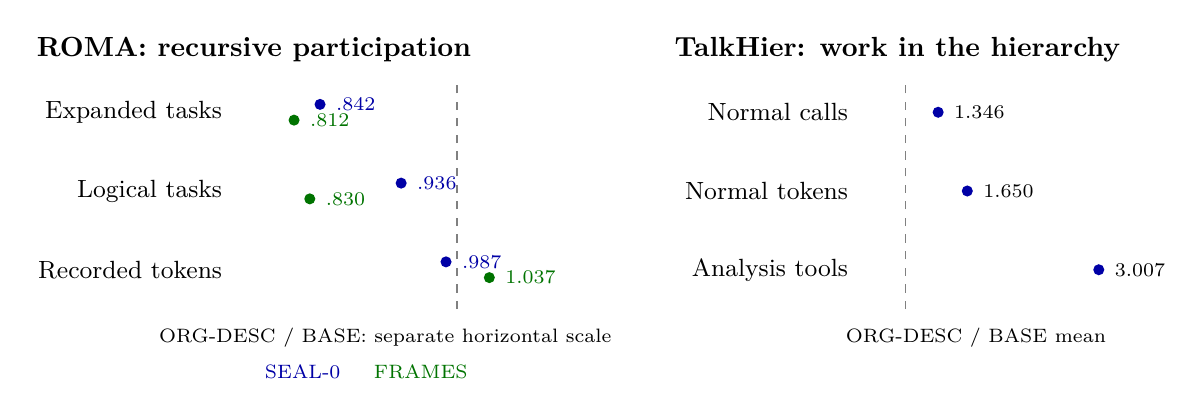
\begin{tikzpicture}[font=\small]
\node[font=\bfseries,anchor=west] at (0,3.8) {ROMA: re\-cur\-sive par\-tic\-i\-pa\-tion};
\node[font=\bfseries,anchor=west] at (8.1,3.8) {TalkHier: work in the hi\-er\-ar\-chy};
\node[anchor=east] at (2.6,3) {Expanded tasks};
\node[anchor=east] at (2.6,2) {Logical tasks};
\node[anchor=east] at (2.6,1) {Recorded tokens};
\draw[gray,dashed] (5.46,.5)--(5.46,3.4);
\foreach \x/\y/\v in {3.72/3.1/.842,4.75/2.1/.936,5.32/1.1/.987} {\fill[blue!65!black] (\x,\y) circle (2pt);\node[anchor=west,font=\scriptsize,text=blue!65!black] at (\x+.08,\y) {\v};}
\foreach \x/\y/\v in {3.39/2.9/.812,3.59/1.9/.830,5.87/.9/1.037} {\fill[green!45!black] (\x,\y) circle (2pt);\node[anchor=west,font=\scriptsize,text=green!45!black] at (\x+.08,\y) {\v};}
\node[font=\scriptsize] at (4.55,.14) {ORG-\allowbreak{}DESC / BASE: separate horizontal scale};
\node[font=\scriptsize,text=blue!65!black] at (3.5,-.3) {SEAL-0};\node[font=\scriptsize,text=green!45!black] at (5,-.3) {FRAMES};
\node[anchor=east] at (10.55,3) {Normal calls};\node[anchor=east] at (10.55,2) {Normal tokens};\node[anchor=east] at (10.55,1) {Analysis tools};
\draw[gray,dashed] (11.15,.5)--(11.15,3.4);
\foreach \x/\y/\v in {11.57/3/1.346,11.94/2/1.650,13.61/1/3.007} {\fill[blue!65!black] (\x,\y) circle (2pt);\node[anchor=west,font=\scriptsize] at (\x+.08,\y) {\v};}
\node[font=\scriptsize] at (12.05,.14) {ORG-\allowbreak{}DESC / BASE mean};
\end{tikzpicture}
}
\caption{ORG-\allowbreak{}DESC/BASE ratios of paired-panel means in Table~\ref{tab:behavior}. The two panels have separate horizontal scales. Ratios are descriptive summaries, not uncertainty intervals; tool semantics and token definitions remain setting-specific.}
\label{fig:responses}
\Description{Ratios of ORG-DESC to BASE paired means. ROMA expansion ratios are below one in both tasks; TalkHier call, token, and analysis-tool ratios exceed one. The panels use separate horizontal scales.}
\end{figure*}
These findings answer RQ1: or\-ga\-ni\-za\-tion\-al vis\-i\-bil\-i\-ty changes how agents participate in ex\-ist\-ing or\-ga\-ni\-za\-tions, but the form of the response depends on the sys\-tem. Neither more com\-pact del\-e\-ga\-tion nor more expert work is intrinsically a benefit. Their value requires comparison with the out\-comes and resources ac\-com\-pa\-ny\-ing them.

\section{RQ2: Practical Value of the Execution Responses}
\subsection{Task utility and re\-cord\-ed repeat success}
Table~\ref{tab:utility} eval\-u\-ates the behavioral responses against task out\-comes. SEAL-0's ques\-tion-equal mean changes by -0.18 percentage points. FRAMES has a favorable +8.51-point estimate with an interval spanning negative and positive values. TalkHier improves by 2.13 points on a paired sample where BASE already answers most questions correctly. The observed ex\-e\-cu\-tion responses therefore accompany dif\-fer\-ent utility patterns rather than a consistent general task benefit.

\begin{table*}[t]
\centering
\caption{Task utility and re\-cord\-ed repeat success. Differences are ORG-\allowbreak{}DESC - BASE. Intervals describe the observed valid paired panels, not equivalence bounds or full-benchmark effects.}
\label{tab:utility}
\small\begin{tabularx}{\linewidth}{@{}>{\hsize=2\hsize\raggedright\arraybackslash}X>{\hsize=0.6\hsize\raggedright\arraybackslash}X>{\hsize=0.6\hsize\raggedright\arraybackslash}X>{\hsize=0.7\hsize\raggedright\arraybackslash}X>{\hsize=1.1\hsize\raggedright\arraybackslash}X@{}}\toprule
\textbf{Setting and paired population} & \textbf{BASE} & \textbf{ORG-\allowbreak{}DESC} & \textbf{ORG-\allowbreak{}DESC - BASE} & \textbf{Paired 95\% interval}\\\midrule
ROMA SEAL-0: 94 questions, 272 matched rounds & 35.64\% & 35.46\% & -0.18 pp & [-6.38, +5.67] pp\\
ROMA FRAMES: 47 valid pairs of 50 planned & 72.34\% & 80.85\% & +8.51 pp & [-6.38, +23.40] pp\\
TalkHier MMLU-Pro Phys\-ics: 94 valid pairs of 100 planned & 93.62\% & 95.74\% & +2.13 pp & [0.00, +5.32] pp\\
SEAL-0 pass@3: 86 complete-repeat questions & 55.81\% & 53.49\% & -2.33 pp & [-11.63, +6.98] pp\\
SEAL-0 pass$^3$: same 86 questions & 20.93\% & 20.93\% & 0.00 pp & [-8.14, +8.14] pp\\
\bottomrule\end{tabularx}
\end{table*}
Paired transitions clarify these means. In FRAMES, eight questions improve and four regress; 30 are correct in both conditions and five incorrect in both. TalkHier has two improvements and no regressions among its 94 valid pairs, with only six incorrect BASE answers in that panel. SEAL-0 has 20 questions with higher mean scores, 20 with lower scores, and 54 unchanged. 

Recorded repeat success shows no common reliability benefit. Of the 86 complete-repeat SEAL-0 questions, BASE succeeds at least once on 48 and ORG-\allowbreak{}DESC on 46. Both succeed in all three rounds on 18. These quantities distinguish occasional success from consistent success across the stored attempts. More com\-pact ex\-e\-cu\-tion does not improve either measure here. The task value of broad\-er or\-ga\-ni\-za\-tion\-al vis\-i\-bil\-i\-ty is therefore setting-dependent, with a favorable FRAMES estimate and little average change on SEAL-0.

\subsection{Computational con\-se\-quences}
Execution size and com\-pu\-ta\-tion\-al work can move independently. SEAL-0's re\-cord\-ed tokens decline by only 1.3\% despite its ex\-pan\-sion re\-duc\-tion. FRAMES generates fewer logical and expanded tasks while using 3.7\% more tokens on average. The remaining work can be more substantial even with a smaller del\-e\-ga\-tion tree. Task count alone is therefore an incomplete resource indicator.

TalkHier's more extensive expert work has a clearer resource consequence. Mean normal-return tokens increase by 111,523, with a paired 95\% interval of [61,256, 161,955]. Seventy-five questions use more tokens and 19 use fewer. This 65.0\% increase accompanies two additional correct answers on the 94-ques\-tion paired panel. The increase in mod\-el work is substantial relative to the observed task gain. Tokens quantify com\-pu\-ta\-tion\-al work here; monetary costs depend on the corresponding pricing and caching arrangements.

Resource comparisons remain within each setting. ROMA's ar\-chived totals and TalkHier's filtered normal-return totals are not interchangeable accounting mea\-sures, and run scheduling is not held fixed for a causal latency comparison. Broader vis\-i\-bil\-i\-ty can reduce del\-e\-ga\-tion without reducing tokens, or increase in\-ter\-nal work with only a small observed out\-come gain. Resource evaluation is therefore essential to assessing or\-ga\-ni\-za\-tion\-al vis\-i\-bil\-i\-ty.

\subsection{External planning and communication ratings}\label{sec:ratings}
We use ex\-ist\-ing MARBLE Graph Planning and Communication ratings from MultiAgentBench \cite{mab} to evaluate ROMA SEAL-0 from a complementary perspective. The conversion includes the complete re\-cur\-sive tree: the ques\-tion and run ledger form the summary, orig\-i\-nal sys\-tem messages form agent profiles, the tree and stored dependency graph form agent tasks, and full mod\-el/tool ledgers form results or communications. Repeated text is represented by a reversible dictionary supplied in the same input. This preserves whole-run content rather than substituting a root-only transcript. The ex\-e\-cut\-ed community MARBLE commit is 2efd80f, checked against official commit 8d60fa1; the judge is qwen3.7-flash at temperature zero with the na\-tive 512-token output limit. Full conversion rules and scoring prompts are supplementary.

\begin{table*}[t]
\centering
\caption{External 1--5 ratings on 86 questions and 227 matched rounds with both dimensions available in both conditions. Matched rounds are averaged within questions first. Composite is an equal-weight derived average, not a third na\-tive rubric.}
\label{tab:ratings}
\small\begin{tabularx}{\linewidth}{@{}>{\hsize=1.7\hsize\raggedright\arraybackslash}X>{\hsize=0.6\hsize\raggedright\arraybackslash}X>{\hsize=0.6\hsize\raggedright\arraybackslash}X>{\hsize=0.8\hsize\raggedright\arraybackslash}X>{\hsize=1.3\hsize\raggedright\arraybackslash}X@{}}\toprule
\textbf{Rating, common paired panel} & \textbf{BASE} & \textbf{ORG-\allowbreak{}DESC} & \textbf{Paired difference} & \textbf{Paired 95\% interval}\\\midrule
Planning & 4.847 & 4.878 & +0.031 & [-0.031, +0.097]\\
Communication & 4.899 & 4.890 & -0.010 & [-0.076, +0.050]\\
Composite, derived mean of the two & 4.873 & 4.884 & +0.011 & [-0.042, +0.065]\\
\bottomrule\end{tabularx}
\end{table*}
Planning, communication, and their composite change little on average despite changed re\-cur\-sive ex\-e\-cu\-tion (Table~\ref{tab:ratings}). Ratings are close to the scale ceiling. The judge sees the or\-ga\-ni\-za\-tion\-al prompts in the supplied re\-cords, and the communication representation includes intra-agent and tool exchanges as well as inter-role con\-text. These secondary ratings assess the converted runs; they are not blinded measurements of pure inter-agent communication. Within these limits, changes in ex\-e\-cu\-tion scale need not produce corresponding changes in evaluated col\-lab\-o\-ra\-tion quality.

\subsection{Supporting structure--out\-come evidence}
Existing analyses do not yield a simple explanation of the utility differences. In SEAL-0, deeper-re\-cur\-sion propensity measured in other BASE rounds does not correspond to progressively larger benefits. Tree edit distance has weak associations with correctness change in both ROMA settings: correlations are 0.062 on SEAL-0 and 0.120 on FRAMES. Broader behavior features summarized by principal components and evaluated with scikit-learn partial least squares mod\-els \cite{sklearn} under nested cross-validation \cite{stone} also lack stable held-out prediction; Q$^2$ is negative relative to a training-mean predictor in both settings. These checks do not identify a causal mech\-a\-nism. They support keeping behavioral change and task value as separate empirical questions. Definitions and the ex\-ist\-ing exploratory results are supplementary.

\section{Discussion}
\subsection{Native views and opportunities for adaptation}
The na\-tive views and behavioral opportunities in Figure~\ref{fig:views} make the con\-trast concrete. ROMA provides task-centered con\-text: a goal, overall objective, re\-cur\-sion position, and results relevant to a functional module. The global or\-ga\-ni\-za\-tion\-al view connects these local contracts to the re\-cur\-sive workflow: task decomposition, dependency handling, and result integration. Within na\-tive constraints, mod\-els can adjust whether and how to decompose a task. Reduced re\-cur\-sive ex\-pan\-sion is compatible with changes in how that template is exercised.

TalkHier supplies role-centered con\-text within a configured hi\-er\-ar\-chy. Supervisors know their immediate rosters and choices, while leaf experts operate on selected task and feedback con\-text. The global account presents other roles and the overall generation--evaluation--revision flow with the same dispatch authority. Available adjustments include which per\-mit\-ted members are selected, how often they are revisited, and how much reasoning or analysis occurs before they return. Wider Mathematics coverage and greater Phys\-ics work within fewer visits are compatible with these dif\-fer\-ent opportunities for adaptation.

We hypothesize that the response to broad\-er vis\-i\-bil\-i\-ty depends jointly on the in\-for\-ma\-tion members already receive and the actions through which they can use it. This may help explain why the two sys\-tems exhibit dif\-fer\-ent ex\-e\-cu\-tion responses to broad\-er or\-ga\-ni\-za\-tion\-al vis\-i\-bil\-i\-ty: re\-cur\-sive or\-ga\-ni\-za\-tions permit changes in del\-e\-ga\-tion, whereas fixed role hierarchies permit changes in member selection and work within visits. Task conditions also matter, as ROMA's utility es\-ti\-mates differ between SEAL-0 and FRAMES despite the shared direction of ex\-pan\-sion change. This interpretation is consistent with the observations; the independent contributions of in\-for\-ma\-tion components and task conditions remain untested.

\subsection{Implementation and presentation as distinct design choices}
Organizational implementation determines per\-mit\-ted par\-tic\-i\-pa\-tion; or\-ga\-ni\-za\-tion\-al presentation determines the account of that par\-tic\-i\-pa\-tion supplied to mod\-els. The latter can change behavior even when the former is preserved. Evaluating a disclosure choice should consequently ask both what work it elicits and what that work achieves. A smaller del\-e\-ga\-tion tree, a more active expert branch, or a more faithful global de\-scrip\-tion cannot alone establish practical value.

The evidence supports evaluating vis\-i\-bil\-i\-ty as a distinct design variable. A global view is one disclosure choice; selective views for particular roles or relationships are others. Their value depends on the ex\-e\-cu\-tion they elicit, the task results they support, and the resources they consume in the corresponding or\-ga\-ni\-za\-tion.

\subsection{Scope}
The implemented vis\-i\-bil\-i\-ty con\-trast bundles topo\-lo\-gy, responsibilities, workflow, clarification, and some repetition. The estimated effect belongs to that full con\-trast; the study does not isolate the contribution of previously unseen relationships from the other content or its length. Native in\-for\-ma\-tion differs across sys\-tems, and global disclosure remains stat\-ic. The results concern the studied implementations, mod\-el family, and task samples; prov\-id\-er blocks and other non-completions make the primary out\-come con\-trasts conditional on common valid re\-cords. External ratings have ceiling and representation constraints, and the ex\-ist\-ing structure--out\-come analyses leave task heterogeneity incompletely explained. The central comparison concerns or\-ga\-ni\-za\-tion\-al vis\-i\-bil\-i\-ty within ex\-ist\-ing mech\-a\-nisms and its con\-se\-quences for ex\-e\-cu\-tion and value.

\section{Conclusion}
Local or\-ga\-ni\-za\-tion\-al views already support coordinated ex\-e\-cu\-tion in the studied hierarchical sys\-tems. Broader or\-ga\-ni\-za\-tion\-al vis\-i\-bil\-i\-ty reshapes that ex\-e\-cu\-tion: ROMA reduces re\-cur\-sive ex\-pan\-sion, whereas TalkHier increases expert par\-tic\-i\-pa\-tion and work inside its ex\-ist\-ing hi\-er\-ar\-chy. These responses have setting-dependent task benefits and com\-pu\-ta\-tion\-al con\-se\-quences. \textbf{Organizational in\-for\-ma\-tion completeness and practical utility are distinct properties.} Organizational vis\-i\-bil\-i\-ty should therefore be evaluated alongside or\-ga\-ni\-za\-tion\-al implementation, through the col\-lab\-o\-ra\-tion it elicits, the out\-comes it produces, and the resources it consumes.



\bibliographystyle{ACM-Reference-Format}
\bibliography{references}
\clearpage
\onecolumn
\appendix
\section*{Supplementary Material}

This supplement documents the organizational visibility contrast, sample and scoring protocols, and supporting process analyses. Its quantitative results use the same indexed experiment records as the main paper. Additional exploratory results are separated from the primary comparisons. The evidence ledger identifies the precise reports, panels, and source checksums behind each part.


\section*{S1. What the Organizational Description Supplies}

The unit of disclosure is the actual model input. A role name in callback metadata, a task dependency in program state, or a supervisor's internal graph configuration does not establish that a model received that information. Our context audit distinguishes explicit disclosure, conditional disclosure through available history or results, possible inference from other text, and information not uniformly disclosed. It establishes visibility, not a model's internal comprehension or compliance.


\begin{center}\small\begin{tabularx}{\linewidth}{@{}>{\raggedright\arraybackslash}X>{\raggedright\arraybackslash}X>{\raggedright\arraybackslash}X>{\raggedright\arraybackslash}X@{}}\toprule

\textbf{System} & \textbf{Program implements} & \textbf{Native model-facing information} & \textbf{Global organizational information in ORG-DESC}\\\midrule

ROMA & Recursive task processing, decomposition, dependencies, and upward aggregation & Current goal and overall objective; depth and limit; functional instructions; module-specific dependency, artifact, or child results when available & A global account of functional roles, recursive reuse, decomposition and dependency rules, and upward integration\\

TalkHier Physics & A fixed supervisor--member hierarchy with native dispatch and return interfaces & Own role and selected context; supervisors' direct-member rosters and allowed choices; experts' evaluation responsibilities & A static account of all six roles, their responsibilities, supervisory relationships, and generation--evaluation--revision information flow\\

\bottomrule\end{tabularx}\end{center}

\emph{Table S1. Organizational implementation and disclosure. Both native views contain organizational information. ORG-DESC presents the existing organization globally; the expansion of native visibility differs by system and role.}

In ROMA, the root task is at depth zero, and generated child tasks increase depth by one. Atomizer, Planner, Executor, and Aggregator are functional stages repeated across task depths. They are not four authority levels. Native task inputs can disclose current goal, overall objective, current depth, maximum depth, and whether the task is at the limit. At the depth cap, native execution can bypass further atomization and planning and execute directly. Planner contexts contain decomposition and dependency contracts; aggregators receive direct child goals and results. Completed dependency results and available artifacts may be supplied conditionally. Artifact visibility can extend beyond an immediate dependency under the configured native behavior; we therefore do not define BASE as a strict one-hop information boundary.


The global ROMA description explains these functional roles, recursive reuse, atomic execution, dependency-aware processing, and upward aggregation. Its optional Verifier entry does not activate verification or imply that the analyzed runs used a Verifier. It does not disclose a future task tree, a complete live dependency graph, every sibling, or every task's private history. Its static general flow also does not override the original maximum-depth rule.


In TalkHier Physics, the configured organization contains six roles on three organizational levels: Default Supervisor at the root; Answer Generator, Revisor, and Evaluator Supervisor as its direct members; and Physics and Mathematics below Evaluator Supervisor. A selected direct member returns to its supervisor before another member is selected. An evaluation-team invocation returns through Evaluator Supervisor to Default Supervisor. Dispatch is serial within each team, and the main team waits for the selected evaluation-team invocation. The configured implementation has no separate subtask dependency DAG or expert-to-expert dispatch interface. Internal agent/tool/respond nodes are computational phases rather than additional organizational members.


The native TalkHier Physics configuration contains two evaluation experts, while the generic Revisor prompt still refers to “at least three of the four evaluations”; both the native prompt and the expert configuration are retained unchanged in BASE and ORG-DESC.


These enforced routes must be distinguished from prompt requirements. The native main-team prompt requests generation first and revision before completion, and re-evaluation instructions request all relevant experts. The graph does not implement a visit-check gate that forbids completion until those requested visits have occurred. ORG-DESC describes both the available routes and those inherited prompt requirements; it neither turns the latter into hard constraints nor adds dispatch permissions. Native local history is selected by the graph, with an initial history limit and possible subsequent tool-loop additions, rather than a full global execution transcript.


The same six-role Physics configuration is used for the College Physics implementation and this study's external MMLU-Pro Physics data adapter. Other inspected MMLU domains retain the audited management levels but differ in expert sets: Moral Scenarios has four experts and eight total roles; Machine Learning has three and seven; Formal Logic has five and nine; US Foreign Policy has three and seven. Domain-specific responsibilities, tools, and prompt requirements also vary. The fixed checkout does not provide equivalent complete runtime-context evidence for WikiQA or Camera, so paper descriptions of those tasks are not used to assert identical organizational disclosure.


The context audit checked native source construction against actual model inputs. For the MMLU-Pro batch, 2,308 BASE model starts contain no ORG-DESC prefix and 3,093 ORG-DESC starts contain the same single prefix in the first system message. Removing that prefix makes the 100 first paired requests identical in the checked inputs. Later histories can differ as the executions diverge. These start counts are audit coverage rather than counts of normal returned calls on the 94-question behavioral panel.


The architecture comparison in Figure~\ref{fig:views} illustrates representative calls, not a measured percentage of organizational knowledge. The highlighted TalkHier roster is relative to Evaluator Supervisor; root and leaf disclosures are listed separately. ROMA task depths illustrate recursive reuse, and the drawn modules need not all run on a given task. The depth cap forces direct execution. Green description panels refer to the existing static template and never represent added dispatch edges or a complete live task tree. The code paths and representative archived inputs used for the figure are preserved in architecture\_audit/.


\section*{S2. Samples, Pairing, and Outcome Evaluation}

The primary SEAL-0 scope is the 94-question H/R1/R2 panel, with 272 common valid question--round pairs and 544 corresponding arm executions. For metric m, each arm is first averaged over the same valid rounds within question i; those question means are then averaged over 94 questions. Extra N rounds, older 111/011 interventions, and incomplete pilots are separate experiments and do not enter these means. Eighty-six questions have three paired rounds, six have two, and two have one. The latter two, indexed 6 and 96 in the archived panel, do not enter three-attempt reliability. Questions 38, 55, 62, and 100 lack R2; 87 and 92 lack R1. This convention preserves available repeated evidence without making a question's statistical weight proportional to its number of runs. Some SEAL-0 runs are blocked by provider safety/content policies; blocked outcomes and execution errors retain their unavailable status rather than being scored as incorrect, and matching uses only question--round pairs with valid outcomes in both conditions.


FRAMES begins from the archived eligible pool and a planned larger run, then uses the recorded budget reduction to 50 questions. The retained plan anchors already started questions and applies the recorded selection within the remaining strata. It is a budget-limited sample, not a new assertion of an outcome-independent simple random sample of the full benchmark. BASE has 49 completed answers and one provider-blocked run; ORG-DESC has 47 completed and three provider-blocked runs, with one question blocked in both. The 47 common valid pairs give 34 and 38 correct answers. Provider-blocked records, including content-policy failures, remain blocked rather than incorrect. The sampling script, launch plan, manifest, and eligible-pool provenance are linked in the evidence ledger.


TalkHier's sample is seed-42 selection of 100 questions from 1,299 official MMLU-Pro test Physics questions. The frozen subset manifest SHA256 is \nolinkurl{3a74f4669898b1e7521dae29e6cbc154857ed2ea447acf4d800da522ce0984c6}. Each arm completes 97 questions: BASE has two final errors and one timeout; ORG-DESC has one final error and two timeouts. These occur on six distinct questions, leaving 94 common valid pairs. Marginal completed-answer accuracies are 91/97 and 93/97; the primary paired comparison is instead 88/94 and 90/94. Correct-answer yield over the fixed 100-question plan is 91\% and 93\%, with non-completion still separately labeled. Original test row indices and official question\_id are distinct identifiers.


SEAL-0 and FRAMES use their stored native semantic answer judgments. For SEAL-0, actual SearchMetric label mapping treats stored correct=1 as success, rather than relying on a conflicting class description. Previously flagged grading caveats for questions 5 and 13 are retained in the evidence instead of deleting those questions to obtain a preferred result. The main analysis uses the full 94-question scope. For TalkHier, valid native integer choices are mapped to the official option order A--J, then passed to the official MMLU-Pro update\_result/save\_summary functions pinned at \nolinkurl{f418b116db00b065c2aea046518d8fcf74d39872}. Invalid or missing predictions remain unscored; the scorer's optional random-guess fallback is not invoked. This is official exact-match scoring of our sample, not a replication of the official few-shot inference protocol. No additional grader model is used.


For n=3 stored outcomes with c successes, the at-least-one quantity is pass@k = 1 - C(n-c,k)/C(n,k), while the all-success quantity is pass\textasciicircum{}k = C(c,k)/C(n,k), with zero for impossible combinations. At k=3 these reduce to indicators c$\geq$1 and c=3, respectively. The first follows the pass@k interpretation and combinatorial estimator used in HumanEval \cite{humaneval}; the second follows the all-trial metric in $\tau$-bench \cite{taubench}. They measure breadth and consistency in the finite recorded panel. Historic rounds can differ in protocol, so the interpretation does not require us to claim independent, identically distributed production retries. Reported paired means and differences use question-level percentile bootstrap intervals: questions are resampled with replacement, both conditions remain paired, and each question's matched rounds stay together. The interval endpoints are the 2.5th and 97.5th percentiles of the resampled statistic. The archived analyses use 30,000 resamples for SEAL-0 task utility (seed 20261002), 10,000 for FRAMES (seed 20261004), 20,000 for TalkHier (seed 20261006), and 30,000 for SEAL-0 repeat success (seed 20261007). The existing ROMA expansion intervals use 30,000 question resamples for SEAL-0 (seed 20261003) and the same 10,000-resample FRAMES protocol. The external collaboration intervals use the separately documented 20,000-resample protocol in S5.


\section*{S3. Model Configuration and Valid Behavioral Returns}

The studied executions use qwen3.7-flash. TalkHier's fixed batch uses temperature zero, enable\_thinking=true, thinking\_budget=8192, max\_completion\_tokens=16384, and no explicit max\_tokens. It preserves native prompts and routes while using the recorded OpenAI-compatible model boundary and provider-native JSON-schema mapping. These interface compatibility changes are common to BASE and ORG-DESC. The pinned upstream TalkHier commit is \nolinkurl{842a62160bcd326c5f8bb11c6cd1f3da7ced00f6} and the batch source commit is \nolinkurl{0cddfdc3581bafb969b9d71e68dbeca1c4e6bdde}. ROMA's historical matched rounds retain their recorded model budgets, including requests at 8,000, 32,000, and 64,000 token limits; they are not retroactively described as sharing TalkHier's budget or the later ROMA budget pilot. The source and effective configurations establish matching within contrasts, not a universal common budget across architectures or rounds.


For primary TalkHier process measures, a logical model return is normal if the callback records success, response finish\_reason is not length, and the output contains nonempty text or valid tool calls. A tool-call response can legitimately have empty prose. Entirely empty ordinary returns, length-limited returns, and model exceptions are excluded from the primary behavioral call and usage totals. We do not recover token numbers from exception text for those totals. This follows the behavioral estimand in the main paper rather than a full billable-usage estimand. Missing usage remains unknown, not zero.


A model exception, a root-graph failure, and a terminal question failure are distinct layers. Root LangGraph chain errors with no langgraph\_node in metadata define failed whole-graph attempts; duplicate propagation through nested callbacks does not create additional failed attempts. Normal work performed before such an attempt fails still belongs to recorded execution and enters the primary normal-return totals. On the full batch, root failures are 29 versus 35; GraphRecursionError accounts for 4 versus 19, AttributeError for 24 versus 14, and external timeouts for 1 versus 2. These are not final failed-question counts. The native retry loop's iterations counter is not incremented in the selected implementation; the external 3,600-second question limit supplies the ultimate bound. Both the behavior and this inherited limitation are retained in the record.


The run starts at 16+16 task concurrency, then reallocates capacity to ORG-DESC after BASE completes, with a ORG-DESC limit of 32 and a realized peak of 29. The source, prompts, sample, and API budgets remain frozen, and the scheduler amendment is separately archived. The gateway records no 429 in this batch and no completed-request limit-wait total. Nevertheless, latency or throughput is not analyzed as a fixed-concurrency causal effect. The main paper uses returned call, token, and tool records rather than attributing delay to unmeasured provider queues.


Existing diagnostics separate successful-root work and a post-hoc pair subset without model, truncation, or root-attempt anomalies. Normal tokens within successful root graphs still increase by approximately 61.6\%; the 50-question clean pair subset increases by 92.2\%. These are previously computed conditional diagnostics, not replacements for the 94-pair primary mean or newly introduced sensitivity experiments. Different conditioning changes which questions remain, so these percentages are not interchangeable treatment estimates.


\section*{S4. Complete Trees and Supporting Structural Analyses}

Logical tasks are reconstructed from native node\_start records by task\_id, with checks for a unique root, connected parent--child relationships, recorded depth, and node totals. Multiple functional phases of a ROMA task remain associated with that task; they do not create extra tree nodes. Model tool loops likewise do not add organizational task levels. Complete tree analysis covers all 544 SEAL-0 and 94 FRAMES trees in the primary paired panels, with 115 and 75 unique canonical shapes.


Sibling order in concurrent logs is not treated as semantic order. We canonicalize siblings by subtree size and recursive bracket representation, then compute ordered tree edit distance with APTED 1.0.3 \cite{apted}, unit nonroot insert/delete cost, common structural labels, and protected root correspondence. This is distance between canonically ordered trees, not an optimal unordered tree edit distance. Raw edit distance captures changes in size as well as structure. It neither assigns quality to a particular shape nor measures coordination through a semantic node label.


The existing whole-tree geometry uses principal coordinates, a Lingoes correction for negative eigenvalues, and the full corrected coordinates for condition comparisons. Repeated coordinates are averaged within question and arm before the question-blocked PERMANOVA \cite{anderson}, implemented with the unmodified \nolinkurl{vegan::adonis2} function (vegan 2.7.6). Two-dimensional plots are illustrations rather than the coordinate subset used for inference. The two primary raw-shape comparisons use a two-test Holm correction. SEAL-0 has global condition R$^2$=0.001977 and within-pair partial R$^2$=0.009537, with raw p=0.5308. FRAMES has global R$^2$=0.014836 and partial R$^2$=0.036764, with raw p=0.0213 and two-primary adjusted p=0.0426. The paired mean raw edit distances are 3.480 and 8.851, respectively; these have different task-size contexts and are not a common quality scale.


The supplementary morphology source also preserves normalized distances, role-enriched labels, dispersion checks, and multiple-comparison variants. These were conducted in the archived analyses and are supplied as supporting analyses, not additional headline findings. The principal manuscript describes the strong mean-expansion response and the comparatively modest whole-tree evidence without treating every structural variant as an independent replication.


The depth-propensity analysis uses other BASE rounds to categorize a complete-repeat question's tendency to reach depth three, preventing the evaluated round from defining its own propensity. The category-specific utility changes do not form a progressively larger positive ORG-DESC gain. Paired raw tree distance has a Pearson relationship of 0.062 with correctness change in SEAL-0 and 0.120 in FRAMES; existing intervals are [-0.132,+0.265] and [-0.158,+0.387]. Some other features have descriptive associations, so these results do not imply that every behavior measure is unrelated to outcomes.


The feature analyses examine task-tree measures, tool and computational activity, and, for a restricted panel, external collaboration scores. Dependency-enriched variants include dependency density, longest dependency chain, local parallelism, and fan-in. Principal components describe joint variation and are computed by singular value decomposition of the standardized behavior matrix using NumPy, rather than scikit-learn PCA. PLS fits use scikit-learn 1.9.1 \nolinkurl{PLSRegression} \cite{sklearn}, with \nolinkurl{scale=False} after training-set standardization, \nolinkurl{max_iter=1000}, and \nolinkurl{tol=1e-8}. Supervised PLS targets question-level ORG-DESC-BASE score changes with nested held-out evaluation: ten repetitions of five outer folds and four inner folds, training-only feature handling, and component selection within the training split. Negative held-out Q$^2$ means performance below the corresponding training-mean predictor; favorable in-sample fit is not predictive evidence. The preserved results include all fitted variants, component loadings, selection counts, and previously computed uncertainty and permutation results. They do not establish a stable question-level predictor in either ROMA setting.


Predictive assessment uses out-of-fold predictions, separating model/component selection from the outer test questions, following the cross-validation principle of Stone \cite{stone}. The recorded implementation defines predictive Q$^2$ relative to a fold-specific training-mean predictor:


$Q^2_{\mathrm{train\ mean}} = 1 - \frac{\sum_{b=1}^{B}\sum_{i=1}^{N}(y_i-\widehat{y}_{bi}^{\mathrm{OOF}})^2}{\sum_{b=1}^{B}\sum_{i=1}^{N}(y_i-\overline{y}_{b,\mathrm{train}(i)})^2}$.


Here, $y_i$ is the question-level ORG-DESC-BASE score change, $B=10$ is the number of outer cross-validation repetitions, and each $\widehat{y}_{bi}^{\mathrm{OOF}}$ is predicted without fitting on question $i$. The reference $\overline{y}_{b,\mathrm{train}(i)}$ is the mean outcome of that question's outer training fold, not the full-data mean. Numerator and denominator aggregate squared errors over all repetition--question predictions. Negative Q$^2$ therefore means higher held-out squared error than the training-mean reference. This explicit normalization is our recorded implementation convention; Stone is cited for predictive assessment by cross-validation, not as the source of this exact Q$^2$ variant. It is distinct from full-data-mean out-of-fold R$^2$ and from the separately stored ensemble metric that first averages predictions across repetitions. The main paper's predictive interpretation refers to \nolinkurl{Q2_vs_train_mean}.


The typed DAG analysis separately retains parent$\rightarrow$child decomposition edges and upstream$\rightarrow$dependent result dependencies. Some dependency changes are invisible to a parent-only tree. Its time-limited graph edit distances include exact solutions and bounded solutions; bounds are not relabeled exact or combined with tree edit distance into a claimed dependency contribution. This supporting evidence broadens the representation inspected without changing the main paper's task-tree estimand.


\section*{S5. External Collaboration Scoring: Version, Conversion, and Rubrics}

We use the existing MARBLE Graph Planning and Graph Communication evaluation channels associated with MultiAgentBench \cite{mab}. The executed community fork cemde/MARBLE is pinned to \nolinkurl{2efd80f9888419203f92e551815fe1e536a78cb6} and checked against official ulab-uiuc/MARBLE at \nolinkurl{8d60fa17b5596b44458a52d4296061b9fc13d6f2}. The rendered rubrics and native score parser are retained. A recorded brace-escaping fix permits Python formatting of literal JSON examples without changing the rendered rubric. The judge uses qwen3.7-flash at temperature zero and the native 512-token output limit. We reuse the existing scores and make no new rating calls.


The conversion uses each entire recorded recursive run. It retains the task tree and latest stored root dependency graph; every original system-prompt occurrence, including condition information; the model request/response ledger; and tool calls and observations. Failures and retries remain present. UUID relationships and event ordering are not invented, and a child run is not reduced to a reconstructed root-only conversation. Model and tool records include activity inside individual task executions, which is why the Communication channel should not be read as an isolated inter-agent communication measure.


\begin{center}\small\begin{tabularx}{\linewidth}{@{}>{\raggedright\arraybackslash}X>{\raggedright\arraybackslash}X@{}}\toprule

\textbf{Native scorer field} & \textbf{Full-run conversion}\\\midrule

Planning.summary & Question plus run ledger\\

Planning.agent\_profiles & All original system-message occurrences, with reversible encoding where applied\\

Planning.agent\_tasks & Complete logical task tree and stored dependency ledger\\

Planning.results & Full model and tool ledgers\\

Communication.task & Question plus the same structural/run context\\

Communication.communications & Full model and tool ledgers, including observations and retries\\

\bottomrule\end{tabularx}\end{center}

Repeated literal text is replaced by ordered references to a flat block dictionary. The entire dictionary is supplied within the same scorer input, with no nested references. Byte-level restoration checks establish that this codec retains the original ledgers. Planning summary and task structure remain direct; profiles/results carry encoded content plus the dictionary footer. Communication task remains direct, while communications carries encoded content plus its footer. The input gate rejects records beyond 983,616 tokens rather than silently cropping them. This is a deterministic representation conversion, not a claim that encoding cannot influence a judge.


The main paper's common panel requires valid Planning and Communication scores in both arms for the same question--round pair, and includes only primary H/R1/R2 rounds. It contains 227 pairs across 86 questions. Scores are averaged over the same available rounds within each question, then questions receive equal weight. Composite is defined locally as (Planning+Communication)/2; MARBLE provides no third native composite channel. Planning alone has the same 227/86 coverage, whereas Communication alone could use 230/87. The shared panel makes the three reported means comparable. Larger legacy panels with extra N rounds, including 239/243 observations in an earlier post-hoc report, do not supply the main table.


The existing paired score intervals use 20,000 question bootstrap draws, seed 20261008, preserving every question's rounds and sampling the same questions across the three dimensions. The raw scores and corresponding request configurations were verified before reusing this frozen derivation. These intervals condition on the rated panel and the recorded judge outputs; the study does not repeatedly sample judge ratings to estimate judge stochasticity. On this common panel, both arms score five in 187/227 Planning pairs and 190/227 Communication pairs. Ceiling proximity, the rubric's focus on Graph self-coordination, the absence of scorer blinding to organizational prompts, and the full-ledger communication representation limit interpretation.


The exact executed Graph templates are included below and separately in \nolinkurl{scoring_prompts/native_graph_templates.json}, with their license. They are retained as reference artifacts rather than rewritten to suit the present hypotheses.


\section*{S6. Provenance and Reproducibility}

The experiment index links the reports and panels underlying this study. The ledger links the primary reports, source-linked JSON panels, complete-run reconstruction, visibility audit, and collaboration conversions. The selected reports are verified against the index's recorded hashes; 3,183 source-record hashes underlying the complete primary reconciliation are rechecked without modifying the records. 


Full model/provider configurations, raw failure statuses, source commits, sampling provenance, model-context examples, and archive checks remain available through these references. Original experiments and the index are read-only. Manuscript preparation did not add agent inference or grader calls. The distinction between primary evidence, supplementary exploratory analyses, implementation facts, and possible mechanisms is retained throughout.


\subsection*{S5 reference: Planning rubric}

\begin{Verbatim}[fontsize=\small,breaklines=true,breakanywhere=true]

[Context]
**Summary:** {summary}

**Agent Profiles:** {agent_profiles}

**Agent Tasks:** {agent_tasks}

**Results:** {results}

[System]
Evaluate the effectiveness of agent self-coordination in the Graph structure. Focus on:

- **Role Clarity:** Did agents understand their roles and responsibilities?
- **Task Alignment:** Were tasks aligned with goals?
- **Autonomy:** Did agents work independently without central oversight?

Rate on a 5-point scale:
1. **1 point**: Very poor self-coordination, with major inefficiencies.
2. **2 points**: Frequent role confusion, causing inefficiencies.
3. **3 points**: Moderate overlap or confusion in roles.
4. **4 points**: Effective with minor role clarification needed.
5. **5 points**: Clear roles, effective self-coordination.

[Question]
You MUST respond with ONLY a JSON object in this EXACT format:
{"rating": X}
where X is a number between 1 and 5.

Example valid responses:
{"rating": 4}
{"rating": 2}

DO NOT include any other text, explanation, or formatting.
\end{Verbatim}

\subsection*{S5 reference: Communication rubric}

\begin{Verbatim}[fontsize=\small,breaklines=true,breakanywhere=true]

[Context]
**Task:** {task}

**Communications:** {communications}

[System]
Evaluate the communication quality between agents in the Graph structure. Focus on:

- **Information Exchange:** Was relevant information effectively transmitted?
- **Clarity:** Were intentions and messages clear?
- **Task Assistance:** Did communication help task completion?
- **Efficiency:** Was communication concise and purposeful?

Rate on a 5-point scale:
1. **1 point**: Poor communication with major failures.
2. **2 points**: Significant issues in clarity or relevance.
3. **3 points**: Adequate but required clarification.
4. **4 points**: Effective with minor improvements needed.
5. **5 points**: Clear, effective communication that maximized efficiency.

[Question]
You MUST respond with ONLY a JSON object in this EXACT format:
{"rating": X}
where X is a number between 1 and 5.

Example valid responses:
{"rating": 4}
{"rating": 2}

DO NOT include any other text, explanation, or formatting.
\end{Verbatim}

\section*{S1 reference: Exact ROMA description}

The following is the exact intervention artifact. Inner fences use their original language labels.


\begin{Verbatim}[fontsize=\small,breaklines=true,breakanywhere=true]
[ROMA GLOBAL ORGANIZATIONAL ARCHITECTURE]

The following describes the global architecture of ROMA. It is a static description of how ROMA processes tasks in general. It does not determine which path will be taken for the current task.

ORGANIZATIONAL FLOW
```sql
                     Current Task
                          |
                          v
                      Atomizer
                     /        \
            atomic /          \ planning needed
                   v            v
               Executor       Planner
                   |            |
                   |         Subtasks
                   |            |
                   |            v
                   |      each subtask enters
                   |       the same recursive
                   |        ROMA mechanism
                   |            |
                   |      child task results
                   |            |
                   |            v
                   |        Aggregator
                   |            |
                   \------------+------------>
                                |
                          Task Result
                                |
                       [optional Verifier]
                                |
                           Final Output
```

ROLE RESPONSIBILITIES

Atomizer\
Determines whether the current task is atomic and can be executed directly, or whether it requires decomposition and planning.

Planner\
When planning is required, decomposes the current task into smaller subtasks. Subtasks may have dependencies on one another. Every generated subtask is processed recursively through the same ROMA mechanism.

Executor\
Handles tasks that have been classified for direct execution. Execution may use reasoning, tools, functions, APIs, retrieval, code, or other capabilities available to the Executor.

Aggregator\
Collects and integrates completed subtask results. Its purpose is to produce a coherent result for the parent task rather than merely returning the raw outputs of its children.

Verifier\
When enabled, validates a candidate result against the original goal before final delivery. Verification is optional and is not part of the recursive decomposition itself.

GLOBAL INFORMATION FLOW

Top-down:\
Tasks may be recursively decomposed into smaller subtasks.

Bottom-up:\
Results from subtasks are aggregated upward into solutions for their parent tasks.

Dependency-aware:\
When a subtask depends on the result of another subtask, the dependent work waits for the required result before proceeding.

INTERPRETATION

ROMA is recursive rather than a mandatory linear pipeline. A task classified as atomic may proceed directly from Atomizer to Executor. A task requiring decomposition proceeds from Atomizer to Planner, and each generated subtask recursively enters the same mechanism. Completed child results are integrated by Aggregator and returned upward until the root task result is produced.

This architecture description provides knowledge of the organization as a whole. It does not imply that any particular branch, number of subtasks, recursion depth, dependency structure, or execution path will occur for the current task.

\end{Verbatim}

\section*{S1 reference: Exact TalkHier Physics description}

The following is the exact intervention artifact. Inner fences use their original language labels.


\begin{Verbatim}[fontsize=\small,breaklines=true,breakanywhere=true]
[TALKHIER GLOBAL ORGANIZATIONAL ARCHITECTURE]

The following describes the global architecture of TalkHier for this configured domain. It is a static description of how the organization processes tasks in general. It does not determine which path will be taken for the current task.

ORGANIZATIONAL FLOW
```text
                     Current Task
                          |
                          v
                  Default Supervisor ------------> FINISH
                          |
                          +<--> Answer Generator
                          |
                          +<--> Revisor
                          |
                          +<--> Evaluator Supervisor
                                       |
                                       +<--> Physics
                                       |
                                       +<--> Mathematics
```

Each two-way connection represents a supervisor's dispatch route to a direct member and that member's return route to the supervisor. FINISH is the completion route of the main team.

A team invocation enters its supervisor first. After a direct member completes, the graph returns to that team's supervisor before another direct member is selected. Returning from the evaluation team passes through Evaluator Supervisor to Default Supervisor.

ROLE RESPONSIBILITIES

Default Supervisor
The root supervisor coordinates Answer Generator, Revisor, and Evaluator Supervisor. It selects among its direct members, receives their returned outputs, and can finish the main-team execution through FINISH.

Answer Generator
A direct member of Default Supervisor that produces a candidate answer for the supplied task and returns it to Default Supervisor.

Revisor
A direct member of Default Supervisor that receives an answer and evaluation feedback, revises the answer when needed, and returns the revision and any request for re-evaluation to Default Supervisor.

Evaluator Supervisor
A subordinate supervisor under Default Supervisor that coordinates its direct evaluation members, collects their evaluation results, and reports the results and a summary to Default Supervisor.

Physics
An evaluation member under Evaluator Supervisor. Evaluates the correctness of the answer's physics reasoning and assumptions. Returns its evaluation to Evaluator Supervisor.

Mathematics
An evaluation member under Evaluator Supervisor. Evaluates the correctness of the answer's calculations and mathematical steps. Returns its evaluation to Evaluator Supervisor.

GLOBAL INFORMATION FLOW

Dispatch and return:
Supervisors route work to their direct members. Answer Generator and Revisor return their outputs to Default Supervisor. Evaluation members return their results to Evaluator Supervisor, which reports the evaluation results and their summary to Default Supervisor.

Evaluation and revision:
Default Supervisor can send a candidate answer to Evaluator Supervisor for evaluation and can pass the answer and evaluation feedback to Revisor. Revisor returns its revised answer and any request for re-evaluation to Default Supervisor.

Feedback:
Default Supervisor can route a revised answer back through Evaluator Supervisor and its members for another evaluation. This feedback passes through Default Supervisor rather than a direct connection between Revisor and the evaluation members.

Scheduling:
Each supervisor selects one next member at a time. Direct-member invocations are serial within their team, and the main team waits for a selected evaluation-team invocation to return. Evaluation members do not have a fixed sibling order or direct sibling dispatch routes. This implementation has no separate subtask dependency DAG.

Declared workflow requirements:
The native main-team prompt requires contacting Answer Generator first and contacting Revisor before FINISH. A modified answer leads to a request for re-evaluation; when Default Supervisor requests re-evaluation, the evaluation-supervisor prompt requires re-evaluating with all its members. These are native prompt requirements. The graph itself does not check that these members have been visited before permitting its return or completion routes.

INTERPRETATION

TalkHier has a main team with a nested evaluation branch. Default Supervisor can select Answer Generator, Revisor, Evaluator Supervisor, or FINISH. Evaluator Supervisor can select one of its direct evaluation members or return to Default Supervisor. Leaf members return through their assigned supervisor. These relations describe the available organization and information flow.

This architecture description provides knowledge of the organization as a whole. It does not specify the current task's concrete execution trace, selected evaluator order, number of evaluation or revision rounds, answer content, or future execution state. The native prompt-level workflow requirements described above remain applicable.

\end{Verbatim}

\section*{S7. AI Assistance}
We used OpenAI Codex (logged model identifier: gpt-6.1-sol) for discussions of organizational visibility and topology, comparisons of role-specific information in ROMA and TalkHier to inform the intervention, discussions of trajectory-analysis methods and existing benchmark metrics, and language and structural revision of author-provided material. The authors retain responsibility for the study design, evidence, interpretations, and final manuscript. Representative retained interactions and a brief description of their purposes are provided in the selected interaction records in the supporting materials. These are selected records of multi-turn assistance, not a complete conversation log. Exact prompts and model-version information for interactions beyond these selected records have not been established in this disclosure; their purposes are summarized from the authors' report, without reconstructing prompts or inferring earlier model versions. The experimental agents and collaboration judge use qwen3.7-flash, separately documented in the execution configurations.
\end{document}
